\subsection{Government Types Of The World (Grafdatabase)}

Begynner med å lese csv filene. Merk at i dette datasettet er det 4 forskjellige csv-filer.

\FigureCounter
\begin{figure}[H]
    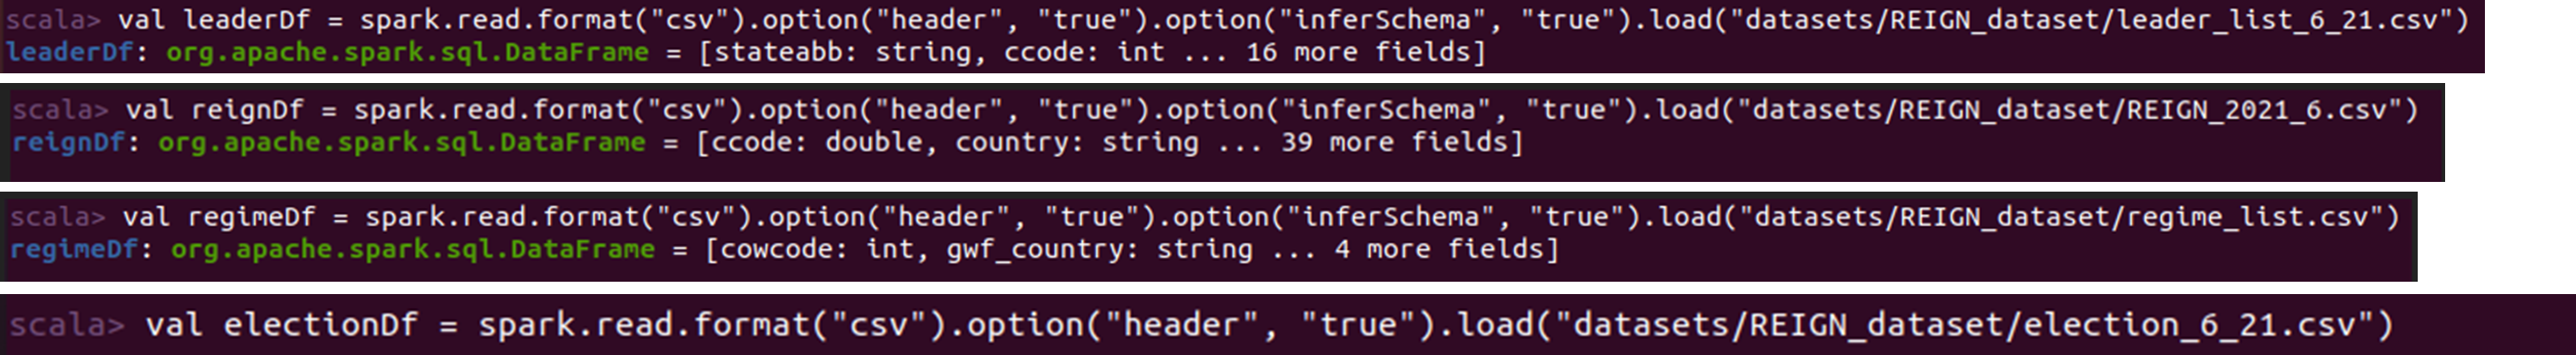
\includegraphics[width=\textwidth]{images/milepael5/graphDbImport.png}
\end{figure}

Så skrive de til parquet filer.

\FigureCounter
\begin{figure}[H]
    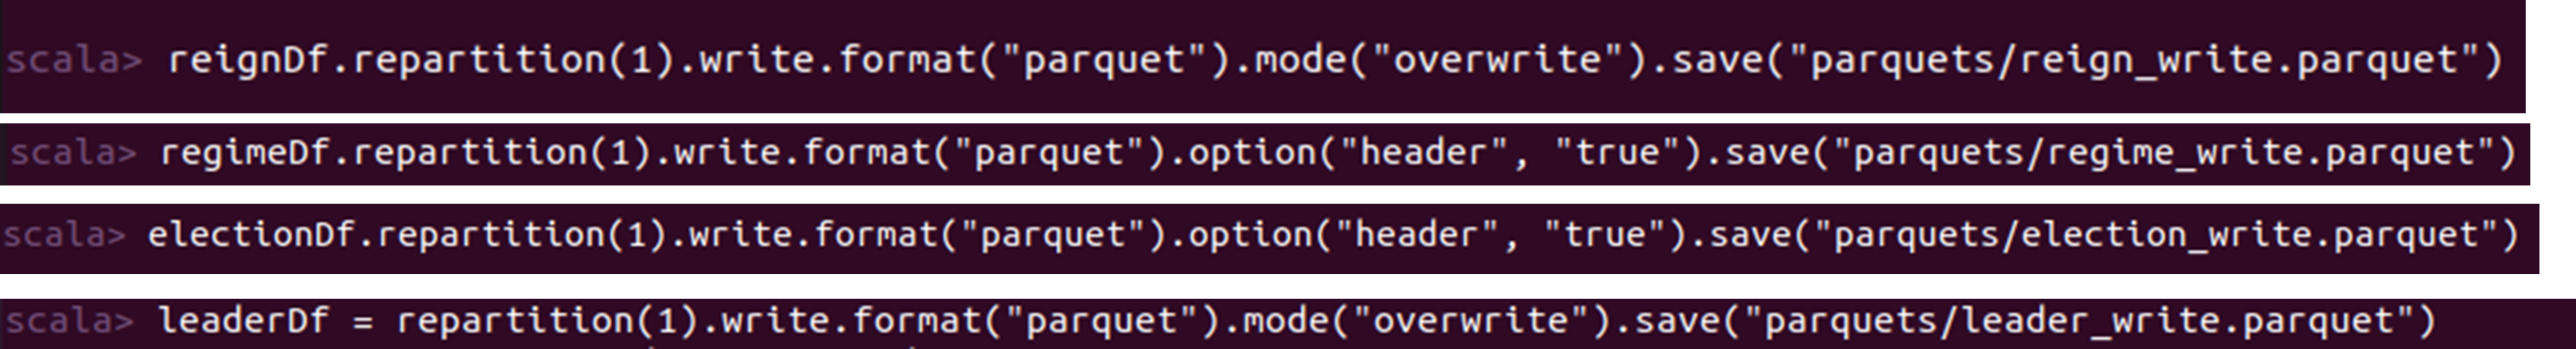
\includegraphics[width=\textwidth]{images/milepael5/writeGraphDb.png}
\end{figure}

\subsubsection{Første Aggregering}
Her lagde jeg kun en aggregering, men til prosjektinnleveringen vil vi bruke de andre også. Aggregeringen viser hvordan hver styremåte har utviklet seg i popularitet gjennom årene. Den opprinnelige skissen fra milepæl 4 ser slik ut:

\FigureCounter
\begin{figure}[H]
    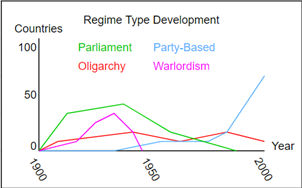
\includegraphics[width=\textwidth]{images/milepael5/regimeTypeGraphic.png}
\end{figure}

Til å begynne med, tenkte jeg å gruppere først på år, så på styremåte, og dermed telle antall opplistinger.

\FigureCounter
\begin{figure}[H]
    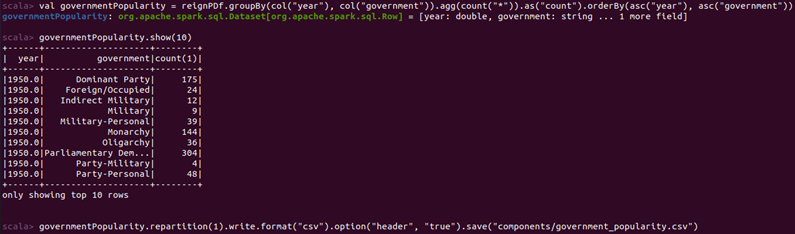
\includegraphics[width=\textwidth]{images/milepael5/governmentPop.png}
\end{figure}

Men dessverre var ikke dette optimalt for lesing av grafiske programmer (excel, libreoffice). Så jeg bestemte meg for å gjøre om på komponenten. I denne nye versjonen har jeg en kolonne for år, og en kolonne for hver styremåte. Da ble aggregeringen slik:

\FigureCounter
\begin{figure}[H]
    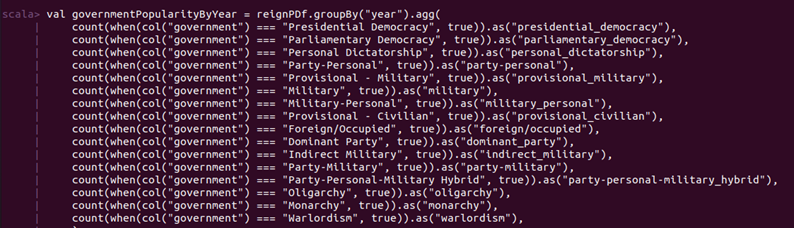
\includegraphics[width=\textwidth]{images/milepael5/govPopByYear.png}
\end{figure}

Framstilling i libreoffice:

\FigureCounter
\begin{figure}[H]
    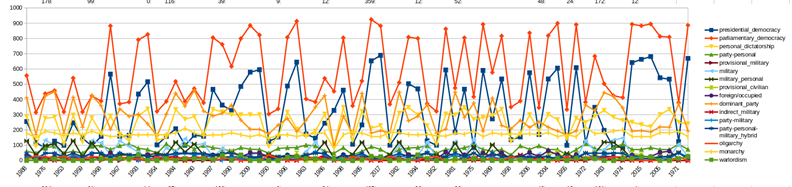
\includegraphics[width=\textwidth]{images/milepael5/libreOfficeGovPop.png}
\end{figure}